\chapter{Introduction}

\section{How it started}

The first Peanuts comic strip appeared in seven U.S. daily newspapers on
October 2, 1950.

\subsection{Charlie Brown}

Charlie Brown is introduced as ``Good Ol' Charlie Brown.''

\begin{figure}
\centering
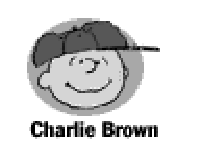
\includegraphics{charliebrown.pdf}
\caption{Charlie Brown}
\end{figure}

\subsection{Snoopy}

Snoopy\index{Snoopy} appears two days later, on October 4. He appears in many later comic
strips. \cite{beingdog}

\begin{figure}
\centering

\includegraphics{snoopy.pdf}
\caption{Snoopy}
\end{figure}

In Chapter \ref{FAQ}, we will learn more about these and other Peanuts.

\section{The mathematics behind first appearances}

The mathematical significance clearly follows from  table~\ref{T:FirstAps} on
page \pageref{T:FirstAps}.

\begin{table}
\begin{tabular}{ll}
Charlie Brown & October 2, 1950\\
Snoopy & October 4, 1950\\
Violet & February 7, 1951\\
Schroeder & May 30, 1950\\
Lucy & March 3, 1952\\
Linus & September 19, 1952\\
Pig-Pen & July 13, 1954\\
Peppermint Patty & August 22, 1966\\
Woodstock & April 4, 1967\\
Snoopy's Father & June 18, 1989\\
Snoopy's Mother & July 26, 1996\\
Joe Cactus & December 8, 1998
\end{tabular}


\caption[Dates of first appearance of characters]{Dates of first appearance of
select Peanuts characters. Source: FAQ of alt.comics.peanuts newsgroup.\\
{\em http://www.peanutscollectorclub.com/peantfaq.txt}}
\label{T:FirstAps}
\end{table}



